\subsection{Visualization}
\label{sec:hard_cut_visualization}

After having implemented the ideas presented in~\ref{sec:hard_cut_approach}, the results were not breathtaking.
Therefore we wanted to receive a feeling for the flaws in our approach by visualizing the features and the decisions that the SVM made.
To make the visualization explorable and interactive, we build a web app written in \emph{HTML} and \emph{JavaScript} using the visualization framework \emph{d3}\footnote{\url{http://d3js.org/}}.
During hard cut detection, we write a \emph{tsv} file containing all required information, such as the histogram differences, the predicted class, and the actual class for every two subsequent frames.
Then a local webserver is started, which has access to the \emph{tsv} file as well as the video frames.
The visualization can be explored using a web browser (see Figure~\ref{fig:hard_cut_visualization}).

\begin{figure}[ht]
	\centering
	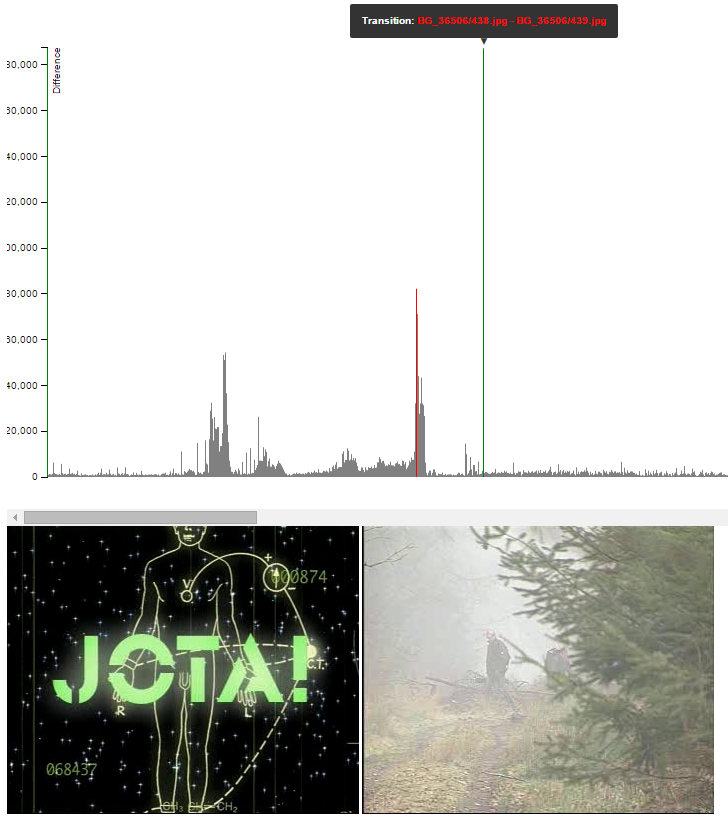
\includegraphics[scale=.5]{images/hard_cut_visualization.png}
	\caption{The height of the bars shows the absolute histogram difference.
    It is calculated by summing up all elements in the histogram difference vector.
    The color of the bars indicates the decision: green -- true positive, gray -- true negative, red -- false positive, orange -- false negative (not in this picture).
    When hovering over the bars, the actual frames are shown below together with a tooltip containing the file names.}
	\label{fig:hard_cut_visualization}
\end{figure}

When inspecting the visualization of a processed video, we can see that the histogram differences are a useful feature for detecting the hard cuts in a video.
In most cases there is one single bar with a high difference surrounded by low differences (see green bar in Figure~\ref{fig:hard_cut_visualization}).
However, we can also see some other peaks that are not hard cuts and are typically surrounded by noisy clusters (see Figure~\ref{fig:hard_cut_noise_visualization}).
Those can be soft cut sequences or just rapid changes during one scene.
Since the SVM just takes the difference between two frames into account, it does not ``see'' the surrounding clusters and therefore makes several mistakes.
Nevertheless, we can improve the classification performance by showing the SVM more soft cuts and frame sequences, where the colors change dramatically.
When learning these negative examples, the decisions made by the SVM are more robust against noisy sequences.
We make fewer mistakes on the noise in Figure~\ref{fig:hard_cut_visualization}, but high peaks, such as in Figure~\ref{fig:hard_cut_noise_visualization}, are still problematic.

\begin{figure}[ht]
	\centering
	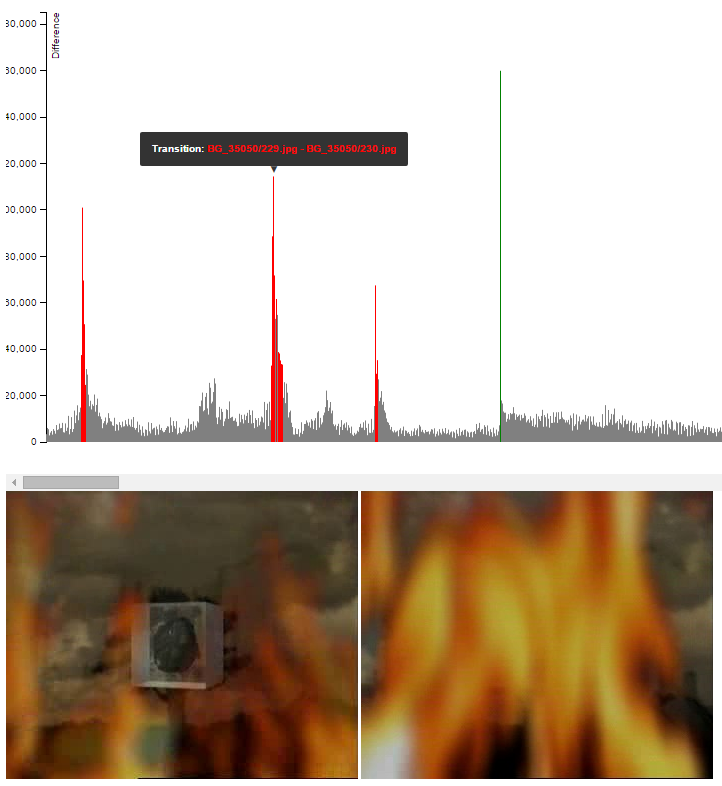
\includegraphics[scale=.5]{images/hard_cut_noise_visualization.png}
	\caption{The histogram differences are problematic when there is lots of noise between two frames. In this case, a burning fire disturbs the classification and introduces lots of false positives.}
	\label{fig:hard_cut_noise_visualization}
\end{figure}
